\documentclass[review]{elsarticle}

\usepackage{lineno,hyperref}
\usepackage{epigraph}
\usepackage{tikz}
\usepackage{subcaption}
\usepackage{standalone}

\usetikzlibrary{bayesnet}
\modulolinenumbers[5]

\journal{New Ideas in Psychology}

%% APA style
\bibliographystyle{model5-names}\biboptions{authoryear}

\begin{document}

\begin{frontmatter}

\title{A communicative approach to early word learning}

%% Group authors per affiliation:
\author{Daniel Yurovsky\corref{mycorrespondingauthor}}
\address{Department of Psychology, University of Chicago, \\5848 S University Ave., Chicago, IL 60637, USA}
\cortext[mycorrespondingauthor]{Corresponding author}
\ead{yurovsky@uchicago.edu}

\begin{abstract}
Young children learn the meanings of thousands of words by the time they can run down the street. Our efforts to explain this rapid development generally begin by assuming that computational-level problem being solved is acquisition. Consequently, we have sought to understand how children infer the meanings of words from cues in the communicative signals of the speakers around them. I will argue, however, that this formulation of the problem is backwards: the computational problem is communication, and language acquisition provides cues about how to communicate successfully. Under this framing, the natural unit of analysis is not the child, but the parent-child dyad. A necessary consequence of this shift is the realization that the statistical structure of the input to the child is itself dependent on the child. This dependency radically simplifies the computational problem of learning and using language.
\end{abstract}

\begin{keyword}
language acquisition, learning, cognitive development
\end{keyword}

\end{frontmatter}

\linenumbers
\renewcommand{\epigraphwidth}{\textwidth}

\epigraph{The infant's Language Acquisition Device could not function without the aid given by an adult who enters with him into a transactional format. That format, initially under the control of the adult, provides  Language Acquisition Support System, LASS. It frames or structures the input of language and interaction to the child's Language Acquisition Device in a manner to "make the system function."}{\cite{bruner1983}}


\section{Introduction}

Humans get a lot of language learning done in strikingly little time. A useful comparison here is the relative rate of two of the most chronicled development milestones: language and locomotion. By the time she is a year old, the typically developing infant is expected to produce several words, and to know the names of many common objects. The same infant is expected to walk while holding onto furniture with only one hand. When this infant develops into a a three-year-old toddler, she will be expected to be able to produce multi-word utterances, understand prepositions (e.g. on, under), and to describe scenes in picture books. This same toddler will also be expected to be able to walk up stairs and stand on one foot for 1 second at a time \citep{squires2009}. There is every reason to think that learning to walk should be a hard problem--it certainly has been difficult to build artificial systems that do it well \citep[e.g][]{collins2005}. However, it is a problem that humans do not seem especially adept at solving relative to other species, particularly in comparison to their clearly unique trajectory in acquiring language \citep{capaday2002,garwicz2009,hockett1959}. Indeed, in the foreword to his seminal book on the topic, \cite{bloom2000} writes that "the child's ability to learn new words is nothing short of miraculous."

So how do we understand our precocious ability to acquire language? For the present paper, let us follow \cite{bloom2000} and focus specifically on learning words. And let us get even more specific: Concrete nouns. Of course, this does not exhaust the space of what children can or do learn in their first few years. But concrete nouns are a useful locus for two reasons: (1) Concrete nouns do make up a large slice of early vocabularies \citep{caselli1995, gentner1982}, and (2) The problem of acquisition should be even worse for more complex and abstract units of language.

\section{The computational problem of language learning}

Although details vary from analysis to analysis, roughly speaking there is broad consensus about the ``computational problem of word learning'' for concrete nouns \citep{marr1982}. The child's is an observer in a world filled with three kinds of observables: words, objects, and referential cues. On any given occasion, the child hears a subset of the words, sees a subset of the objects, and also possibly sees one or more referential cues (e.g. a speaker's gaze) that point to a subset of the objects. The computational problem is to recover from these observables a lexicon--a latent structure that details the mapping between words and objects. The solution to this problem is to resolve the uncertainty about the lexicon by leveraging either the cues available on individual instances, the statistical relationship between words and referents across instances, or both \citep[e.g.,][etc.]{blythe2010, frank2013, kachergis2012, mcmurray2012, siskind1996, yu2008, yurovsky2014}. 

Following this analysis, there is a growing body of experimental evidence that humans--both adults and children--are capable of using exactly this kind of information to learn words. For instance, infants are sensitive to cues like eye-gaze and pointing quite early in life, and can be shown reliably to use them to learn novel words early in the first year of life \citep[e.g.][]{baldwin1993,corkum1998,scaife1975,tomasello2007}. Similarly, adults have been shown to infer word-object mappings from co-occurrence information under a host of different conditions \cite[e.g.][]{vouloumanos2008,yurovsky2013, yu2007}, and many of these experiments have been extended to children and infants as well \citep{smith2008,suanda2014,vouloumanos2009}.

Taken together, these and other similar results are taken as compelling evidence that we are moving in the right direction to understand the rapid pace of children's early word learning. There are skeptical arguments about this framework from the perspective of generalizability--will these same kinds of mechanisms explain the acquisition of verbs or adjectives, for instance \citep[c.f.][]{scott2012}? In this article, I will make a different kind of argument: Our optimism is misguided because of an unlicensed inference from competence to performance \citep{chomsky1965}. These and other demonstrations of early success in learning words from social and statistical cues are evidence of competence, they show that infants \emph{can} learn from these regularities. But they have also been taken as evidence that humans excel at learning from these kinds of regularities, and this inference is unwarranted. Many of these studies demonstrate that human adults are not terribly good at learning words from social or statistical cues. And human children are even worse. 

Let us consider a representative case of social cues: The use of a speaker's eye-gaze to determine the target of her reference. As the title of their landmark paper says, \cite{scaife1975} demonstrate the "capacity for joint visual attention in the infant." Their results show, for instance, that 30\% of of 2-4 month old children follow an experimenter's gaze in one or both trials on which they are tested. Infants do not show success near 100\% until they are a year old. These studies demonstrate capacity, they do not demonstrate excellence. More recent studies using different paradigms show similar results: Young children succeed at above-chance levels, but there is significant development well into late childhood \citep{hollich2000,moore1999,yurovsky2013online,yurovsky2015beyond}. In all of these paradigms, success is defined as the ability to use the speakers' gaze and head direction to distinguish whether she is referring to an object on her left or an object on her right. In more complex visual settings, even older children and adults have difficulty using gaze to infer the target of a speaker's reference \citep{loomis2008,vida2012}.

The pattern of results for statistical word learning is strikingly similar. While infants demonstrate sensitivity to the co-occurrence information between words and objects, their memory for this information is quite fragile even under low levels of ambiguity \citep{vlach2013,vouloumanos2009}. Even for adults this process of statistical inference appears to be highly constrained by limits on memory and attention \citep{smith2011,trueswell2013,yurovsky2015}. In contrast to domains like low-level vision, where human performance is often quite well described by ideal observer models \citep[e.g.,][]{najemnik2005}, human statistical word learning is markedly less efficient than the learning we would expect from a system that made optimal use of the available information \citep{frank2009,yu2012,yurovsky2015}. 

We should not conclude from this data that social cues and statistical cues are not useful for word learning, nor should we conclude that children do not use social cues or do not use statistical information to learn relationships between the words of their native language and the objects in the world. But the discrepancy between children's competence under ideal circumstances and their performance under more challenging circumstances presents: Why do children learn words so rapidly when their learning is so constrained? The solution, I will argue is that our consensus about the computational problem of word learning is incorrect. The right question is not ``how do children learn the meanings words,'' but rather ``how do children and their parents develop systems for communicating successfully'' \citep{bruner1975}. Put another way, we often think of the lexicon as the goal and the communicative moments as the tools through which the lexicon is acquire. I propose that we should make progress instead by inverting this relationship: Communication is the goal, and the lexicon is a tool for successful communication. 

\section{The computational problem of communication}

The computational level description of the word learning implicitly makes strange kind of division: It divorces the problem of learning words entirely from the problem of using them; it assumes that the lexicon is a static property of the external world. That is, that there is some objectively ``right'' mapping between a word and its meaning in the same way that there is a ``right'' way to walk. But these are two very different kinds of problems. The solution for the problem of walking is constrained by biomechanics--the best way to walk is one that minimizes energy expenditure and probability of falling while maximizing distance traversed. Further, the right way to walk does not depend on how other people are walking (at least in the absence of other social goals)--it depends on the infants' developing body \citep{cole2012,garciaguirre2007}. Learning a word is the opposite. The only determiner of the "right" thing to call an object is what other people call it. Language is the solution to a \emph{coordination} problem \citep{chater2010, schelling1980}.

This distinction has profound consequences for how we should think about the word learning problem. One straightforward consequence is that it makes the inductive problem easier by making the learner's biases more likely to be correct. In any learning problem, we are trying to minimize the difference between what is actually true and what we think is true (minimize our prediction error). We minimize this error by using the data available to update our model of the world so that it makes better predictions. But when we do this we always face a tradeoff between to opposing forces: bias and variance \cite{hastie2009}. Variance reflects our sensitivity to the data--the more we let the data influence our beliefs, the more we can fall prey to small fluctuations that can radically change what we think is true (what we sometimes call overfitting). We can reduce our susceptibility to variance by imposing our apriori biases on our model, for instance the preference for parsimony we employ when we remove terms from our regression models that don't meet the the criterion for significance. But these biases reduce our sensitivity to the data, meaning that we will be more resilient to error but slower to learn.

In a coordination problem, to the extent that we are coordinating with people like us, our biases are will tend to be in the right direction. In  natural induction problems, good biases need to be tuned over time by evolution to reflect the structure of the natural world, for instance a bias to prefer face-like patterns over non face-like patterns \citep{johnson1991}. In a coordination problem, our biases do not need to be tuned--they are right no matter what they are. That is because the system being learned is constructed by people who have the same biases as us. While our model of the word learning problem assumes that the relationship between words and their referents is arbitrary, in natural languages this is not the case \citep{saussure1960}. Because our biases are the same as the biases of the other people we are coordinating with, these biases are likely to be reflected in the lexicon. We should thus predict reliable sound-object relationships in the language around us that we essentially get for free--that we don't have to learn \citep{lewis2016,maurer2006,perry2015}. Although there is of course variability in words we use to refer to the same object across language communities, we nonetheless start with a leg-up on total arbitrariness.  

This same consequence of shared-biases is likely to help us in individual learning moments as well. While our models generally assume that the referent is equally likely to be any of the objects around us, in practice this is unlikely to be true. If people talk about the things that they find interesting, and different people find the same things interesting, then we already have a leg up on knowing what object is likely to be referent a speaker's utterance \citep{frank2012,frank2014}.  This shared salience is what drives the strangeness we experience when contemplating \citeauthor{quine1960}'s (\citeyear{quine1960}) problem: We think that `gavagai' means rabbit because rabbit is what we would want to talk about. Of course infants and their parents need not find all of the same things interesting, and they likely do not. But they do share the same goal: The desire to communicate.

\subsection{Language learning in the context of communication}

Because the lexicon was constructed by people, its structure depends on people. And because language is produced by people, the referents also depend on people. These dependencies make the structure of language an easier kind of thing to learn than the structure of locomotion. But the language that an infant hears also depends on them in a more direct way: It is produced to them for motivated reasons. As \cite{gleitman1990} pointed out, the language that children hear is not a veridical running commentary on their visual world; we rarely come home and say ``hello, I am opening the door.'' But neither is language random--it is motivated by the desire to communicate information \citep{grice1969}.

If child-directed speech is intended to communicate information, the referential cues accompanying it should depend systematically on the child. For instance, consider the referential cues like speaker gaze that a child might use to infer the target of a speakers' utterance. We think that these kinds of cues should be informative because speakers are likely to be oriented towards--and looking at--the objects that they are talking about. Indeed, there is a reliable relationship between speaker gaze and referent in analyses of parent-child interactions \citep{frank2013,yu2012embodied}. However, a better predictor of the speakers' reference is where the child herself is looking. Even without following their parents' eye-gaze, children would be right more often than not to just assume that their parents are talking about the object that they themselves are focused on \citep{tomasello1986}. Of course this simple solution would not resolve the discrepant cases, and indeed infants are sensitive to discrepancies between their attentional focus and the focus of their adult interlocutors \citep{baldwin1993}. I mean only to point out that these utterances are fundamentally dependent on the child's own attention, a dependency that does not exist in the standard description of the learning problem.

Similarly, if child-directed speech is goal-oriented, produced in the context of a desire to communicate, it will necessarily have structural features that make it different from the kind structure that our models assume. It should, for instance, be structured in a way that makes it easier to extract the speaker's intended referent. One example of this is that utterance-final words are easier to extract and learn from continuous speech \citep{endress2005,yurovsky2012}. As we would predict, parents tend to place target referents at the end of an utterance, even if this makes an utterance ungrammatical \citep{aslin1996}. Further, we should expect that speech is not uniformly simpler, but that it is fine-tuned to the particular child whose is the recipient of the speech \citep{snow1972}. Recent findings show at least two properties of child-directed speech that are tuned in this way. 

First, one might intuitively predict that the length of child-direct utterances--which serve as a proxy for complexity--might vary monotonically over development. But this turns out not to be the case \citep{newport1977}. However, \cite{roy2009} show in a high-density longitudinal corpus that utterances vary systematically in length around the point in time when the child learns a word. Caregivers' utterances containing a given word (e.g. `fish') follow a U-shaped trajectory centered at the point at which the child learns them. Utterances are at their longest long before the child produces the word for the first time, become shorter in the months before the word is learned, and then lengthen once again. That is, utterances containing a word at their easiest to process right around the period of time when the child is learning them. 

Second, although utterances to young children are not systematically shorter, they are systematically more contingent. \cite{yurovsky2016a} estimated the degree to which parents linguistically align to their developing children--reproducing contingently function word categories in their children's previous utterances. This analysis shows a high degree of alignment early in development that declines steadily over the course of the first 5 years, providing evidence that parents are contingently modifying their utterances on those of their children in a way that supports communication. These findings are consonant with earlier analyses of reformulations and expansions in child-directed speech \citep{chouinard2003,saxton2000}. Parents' speech depends fundamentally on children's own speech in a way that scaffolds them, that maintains a consistent conversation.

Finally, the communicative context of language learning changes not just expectations for input and learnability, but also for what think it means to ``know'' a word. Because our standard computational framework makes learning the lexicon the goal of language acquisition, we test our models by comparing the lexicons they have inferred to a ``gold standard'' lexicon \citep[e.g.,][]{frank2009,fazly2010,yu2008}. And we similarly test our experimental participants' ability to select the right referent when cued with the right word \citep[e.g.,][]{smith2011,yu2007,yurovsky2014}. But this is drastically different from the way that real children's language knowledge is tested. What it means for a child to know a word is for that child to be able to use language to communicate successfully about it's referent. We even know this fact implicitly as scientists. For instance, when we use the MacArthur Child Development inventories to measure children's knowledge. These parent-report vocabulary measures are a standard instrument in the field of developmental psychology, and a tool used by clinicians to assess children's language development. When we ask parents whether their children know the words on these forms, we instruct them that if their child ``uses a different pronunciation of a word (for example, `raffe' for `giraffe' or `sketti' for 'spaghetti'), mark the word right anyway'' \citep{fenson2007}.

The communicative nature of the learning context fundamentally changes the problem being solved. One way of diagramming this change is by formalizing the learning problem in a graphical model--a description of the statistical dependencies between the variables relevant for the learning problem. Figure~\ref{fig:model} shows three such models. In each model, the solid gray circles indicate observed variables--variables whose value that learner can observe directly. The hollow circles show latent variables--variables which have causal consequences for observed variables, but which cannot be observed directly--only inferred from the observed variables. The first model shows the framework implicit in many models of statistical learning. In each situation, the learner observes objects and hears words, and the words come from an unobserved lexicon that is the target of inference. The second model shows a framework proposed by \cite{frank2009} that adds a second latent variable to the situation--the speaker's intention. Inference in this model is more powerful because it leverages a fundamental dependency between ambiguity in individual situations and ambiguity across situations. In each situation, the words a speaker produces are mediated by an intention to refer to only some of the objects. That means that if a learner can discover a speaker's intention, the learner need not consider mappings between the words and any of the unintended objects. This reduces spurious correlations. Similarly, if a learner already knows some mappings, it is easier to discover a speaker's intention--because the learner can make a good guess about which object is being labeled. The third model instantiates the proposal in this article. In this model, the learning situation consists not just of a speaker, but rather a dyad--a parent and a child. Critically, the parent's intention to refer depends not only on the objects, but also on the parent's inferences about the child's intentions. The parents goal is to communicate information that is interesting to the child, and thus a parents' intentions are partially predictable from a child's own words and intentions. Learning in this framework is even easier.


\begin{figure}[tb]
   	\centering
    \begin{subfigure}[b]{0.2\textwidth}
    	\centering
        \resizebox{\linewidth}{!}{\begin{tikzpicture}[]
  
  \node[obs,] (W) {$W$};
  \node[latent, left = 1 of W] (L) {$L$};
  \node[obs, above = 1 of W] (O) {$O$};


  \edge{O}{W};
  \edge{L}{W};


  \plate {S} {(O)(W)} {$S$}
  

\end{tikzpicture}}  
    \end{subfigure}
   	\hfill
    \begin{subfigure}[b]{0.2\textwidth}
    	\centering
        \resizebox{\linewidth}{!}{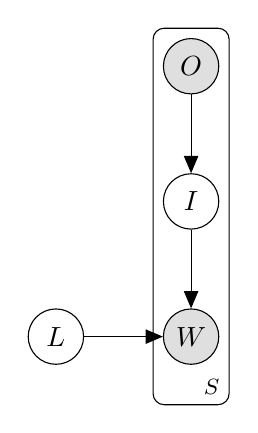
\begin{tikzpicture}[]
  
  \node[obs,] (W) {$W$};
  \node[latent, left = 1 of W] (L) {$L$};
  \node[latent, above = 1 of W] (I) {$I$};
  \node[obs, above = 1 of I] (O) {$O$};


  \edge{O}{I};
  \edge{I}{W};
  \edge{L}{W};

  
  \plate {S} {(O)(I)(W)} {$S$}
  

\end{tikzpicture}}  
    \end{subfigure}
    \hfill
    \begin{subfigure}[b]{0.3\textwidth}
    	\centering
        \resizebox{\linewidth}{!}{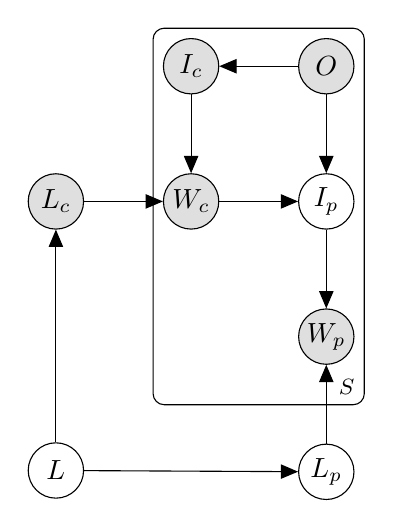
\begin{tikzpicture}[]
  
  \node[obs,] (Wc) {$W_{c}$};
  \node[obs, left = 1 of Wc] (Lc) {$L_{c}$};
  \node[obs, above = 1 of Wc] (Ic) {$I_{c}$};
  \node[obs, right = 1 of Ic] (O) {$O$};
  \node[latent, right = 1 of Wc] (Ip) {$I_{p}$};
  \node[obs, below = 1 of Ip] (Wp) {$W_{p}$};
  \node[latent, below = 1 of Wp] (Lp) {$L_{p}$};
  \node[latent, below = 2.7 of Lc] (L) {$L$};

  \edge{O}{Ic};
  \edge{Ic}{Wc};
  \edge{Lc}{Wc};
  \edge{Wc}{Ip};  
  \edge{Ip}{Wp};
  \edge{Lp}{Wp};
  \edge{O}{Ip};
  \edge{L}{Lc};
  \edge{L}{Lp};

  
  \plate {S} {(O)(Ic)(Wc)(Ip)(Ic)(Wp)} {$S$}
  

\end{tikzpicture}}  
    \end{subfigure}
   	

  \caption{Three computational-level descriptions of language acquisition. In the left-most model, each situation ($S$) contains some observed objects ($O$) that generate observed words ($W$) by their mapping through an unobserved lexicon ($L$). This is the framework implicit in many statistical approaches to word learning \citep[e.g.][]{siskind1996,yu2008,yurovsky2014}. In the middle model, words are generated by an unobserved intention ($I$) on the part of the speaker. This model allows the learner to leverage the inherent synergy between resolving uncertainty in-the-moment and uncertainty across multiple instances \citep{frank2009}. The right model incorporates the communicative nature of the learning situation, noting that the parents' intention ($I_{p}$) depends not only on the objects, but also on their inferences about what the child is interested in (through their observed words $W_{p}$). The child in this model could learn by leveraging this information. Note that the child's lexicon ($L_{c}$) and intention ($I_{c}$) are observable to the child, even though they are not observable to the parent.}
  \label{fig:model} 
\end{figure}


\subsection{Optimal for communication need not be optimal for learning}

I have argued in this paper that much of the credit for children's rapid word learning is due to parents rather than to children themselves. This is because the language that the child is learning is fundamentally dependent on the child, both in the indirect sense that the target lexicon depends on people with the same biases, and in the more direct sense that the input the child hears depends on the parent's inferences about the child's intentions in the moment. The second half of the argument requires that the child's caregiver have a goal that makes the child's process of learning easier: The goal to communicate information. Because the child will need to be scaffolded for communication to succeed, language input will be easier to learn from. 

Importantly, although the parent's speech needs to be goal directed, the goal does not need to be teaching. There may well be times when the parent's goal is to teach the child words, and these times are likely to be particularly informative about the meanings of words. Speech that is pedagogical licenses even stronger inferences because absence of evidence can be taken to be evidence of absence. For instance if the parent chooses examples of a category with the intention to teach, these examples can license strong inferences about the extent of that category \citep[e.g. a parent would be unlikely to choose three peppers to teach the child \emph{vegetable};][]{xu2007}. Parents, particularly of children from some cultural backgrounds, may be motivated by pedagogical goals often, and children might be particularly adept at inferring when parents have these goals \citep{csibra2009}. But the argument in this paper does not require this strong assumption.

Indeed, there are many cases where optimizing for learning and optimizing for communication will be at odds \citep{kirby2015}. Much of the early enthusiasm for the hypothesis that parents tune their speech in a way that helps children ran aground of this phenomenon. For instance, while parents will provide corrective input when children make semantic errors (e.g. calling a \emph{dog} `horse'), they will tend not to provide straightforward corrective signals for syntactic errors. This is because semantic errors can produce failures in in the communication, but syntactic errors generally do not \citep{newport1977}. This is also why parents do not use globally simpler words with younger children--most of the words we use in typical communicative contexts are simple, and their goal is not to optimize for their child's learning \citep{hayes1988,yurovsky2016a}. 

If child-directed speech were optimized for learning, it would certainly make learning easier. But we should not take evidence that speech is not optimal for learning as evidence that it is not \emph{better} for learning than it would be if it were not communicative \citep{eaves-jr2016,mcmurray2013}. Coordinating in-the-moment is only a piece of the language learning puzzle, but it is an important one \citep{tomasello2000}. Understanding how both parent and child contribute to this coordination is critical for understanding why children's language learning is so rapid despite the gap between their competence and their performance in many of the relevant cognitive processes. In the final section, I flesh out this case, providing an example of a simpler computational problem that makes it easier to see why optimal for communication can be different from optimal for learning, but nonetheless be much better for learning than we would expect.

\section{The computational problem of searching an array}

As an analogy, let us consider a simpler model system: The problem of searching an array. Suppose that you have been given an array of integers of some length $n$. And suppose that you can look at any of the integers you want one at a time. You are then asked about some particular integer $i$, and your goal is to determine whether $i$ is somewhere in your array. How difficult would that be? 

Let us consider first the worst case scenario. The worst thing that could happen is that you have to look at every number in the array exactly once. No matter what strategy you have for checking the indices of the array--no matter the algorithm--the number could always be in the last place you look. If you start at the beginning, the number could be at the end. If you start at the end, the number could be at the beginning. And you can never stop early, because if there are any indices you haven't look at yet, $i$ could be in one of them. Therefore, the computational problem of searching this kind of array is said to have complexity of $O\left(n\right)$--it scales linearly with the length of the array. This kind of worst-case analysis is often brought to bear in our descriptions of language as an adversarial problem, one in which the world is as unhelpful as possible \citep[e.g.][]{gold1967, blythe2010}.

In contrast, consider the best case scenario. Suppose that the person who gives you the array and asks you the question is one and the same, and they also know your search strategy. In that case, they might pick an order for the items in the array that makes the very first place you look the only index you need to examine. Either the number they are looking for is in that first index, and you can say yes. Or it is not, and you can say no, knowing that it is also not in any of the other indices. In this case, the length of the array does not matter, and the problem is said to have a complexity of  $O\left(1\right)$--it is a constant difficulty no matter how many numbers are in the array. This is the kind of best-case analysis involved in descriptions of language as pedagogy--analyses under which the adult's goal is to structure input to maximize learning \citep{bonawitz2011, csibra2009, shafto2012}.

Finally, let us imagine a third alternative. Suppose we make one key change in the set up of the problem: The array of integers you get is always sorted in ascending order. Now the worst case is less bad, because you can apply a novel strategy: Binary search. You begin by looking at the integer in the middle of the array (index $\frac{n}{2}$). If this is larger than the number you are looking for, you no longer have to look at any of the numbers to the right of it. If it is smaller than the number you are looking for, you no longer have to look at any of the numbers to the left of it. You can then apply this strategy recursively, finding the number in the middle of the remaining half, again removing from consideration half of the remaining numbers. Now this problem is much easier. Even in the worst case, the number of indices you need to look at scales in the log the length of the array: $O\left(log_{2}n\right)$ \citep{knuth1998}.  

Suppose that we examine a searcher who operates under this last regime, but think we are in the first regime. Several conclusions immediately follow. First, we will think that the searcher is incredibly fast when we observe its searching in its natural regime. Second, when we examine it empirically with unsorted arrays, we will find that the searcher is not terribly good at searching, and we will scratch our heads about why the searcher is so effective in its own environment while being so poor in ours. Finally, we will look to see if worst case analysis is inappropriate, if maybe the person posing the questions in the natural environment is posing them in a way to make search optimally easy (regime 2). We will discover that the answer to this question is no, and we will be left with precisely the paradox with which I began this paper. I argue that this exactly the place in which we find ourselves in our formal analysis of how children learn the meanings of words.

\section{Conclusion}

Young children learn the meanings of thousands of words by the time they can run down the street\citep{mayor2011}. The computational problem they solve is daunting: extracting discrete word forms from a sequence of continuous speech signals and mapping these forms onto their meanings. The explanation for this rapid learning has tended to come in the form of an appeal either to an precocious capacity to use social cues to rapidly infer speakers' intended meaning, or alternatively to a powerful capacity to learn from statistical relationships between words and objects in the world. Yet, the same children who solve this problem continuously forget where they left their coats and hats. How do children learn language so quickly despite their cognitive constraints? 
 
I propose that this paradox arises from a failure to consider a second critical part of the language learning system: The parent. Although children are inundated with language from many sources--including overheard speech--much of their learning seems to be driven by the portion of their language input that is child-directed \citep{weisleder2013}. The structure of this speech is different in a fundamental way than overheard speech, not just because it is in some ways simpler, but also because it depends on the child herself. Language directed at the child is purposeful--it is intended to communicate. If children are aware that this speech is communicative, their learning problem is radically simpler. Because children appear to be sensitive to the communicative nature of speech from quite early on, there is reason to be hopeful that this framework will give a wedge into resolving our paradox \citep{vouloumanos2012,vouloumanos2014}. If there's anywhere in language acquisition we should look for optimality, it is not in the child's head, but in the coordination of the child-parent system.

\section*{References}

\bibliography{newideas}

\end{document}